\documentclass{article}
\usepackage{geometry}
\usepackage{siunitx}
\usepackage{amssymb, amsmath}
\usepackage{booktabs}
\usepackage{hyperref}
\usepackage{float}
\usepackage{graphicx}
\graphicspath{ {../figures/} }

\bibliographystyle{abbrv}

\title{DS3613 Semester Project Report\\
	\em{A Comparitive Analysis of Information Propagation in Blockchain Networks}
}

\author{Yojit Kumar (20231289)\\
  Supervisor: Dr Kalpesh Kapoor}
\date{}

\begin{document}
\maketitle

\section{Introduction}
My interest in this project originates from the problem of epidemic modelling. I am specifically interested in learning how information, diseases, or disturbances propagate through a network of interacting agents. Gossip protocols borrow directly from the mathematics of epidemic modelling (the SIR and SI models) and provide a principled way to study this class of problem in distributed and decentralised computational systems like \textit{Blockchains}. Blockchains, with their large-scale, heterogeneous, and adversarially contested peer-to-peer (p2p) networks, present a particularly rich and complex instance of this propagation problem. This report documents my work so far: a literature survey of how information propagation works in blockchain networks, a description and analysis of the foundations of representative protocols, and a proposal for a hybrid algorithm idea with implementation and experimental validation.

\subsection{Blockchains \& Broadcast Protocols}
A blockchain is a distributed, append-only ledger that records transactions across a peer-to-peer network without relying on a central authority. As first described in the Bitcoin white paper, each block contains a cryptographically verified batch of transactions along with the hash of the preceding block, forming an immutable chain~\cite{nakamotoBitcoinPeertoPeerElectronic2008}. Because each node in the network maintains a complete replica of this ledger, every new block that is mined must be propagated to all participants so that their local copies remain synchronised. The fundamental guarantee that makes blockchain useful is that all honest nodes eventually agree on the same transaction history~\cite{deckerInformationPropagationBitcoin2013}.

The mechanism by which this synchronisation happens is the broadcast protocol, sometimes called a dissemination or propagation protocol. A broadcast protocol governs the rules by which a message (block/transaction) originating at one node is relayed through the network until it reaches all other nodes~\cite{deckerInformationPropagationBitcoin2013}. In Bitcoin's original implementation, this is accomplished through a gossip-style protocol: upon receiving and verifying a block, each node announces its availability to neighbouring nodes via an inventory (\textit{inv}) message; neighbours that do not yet have the block respond with a \textit{getdata} request, and the block is then transferred~\cite{deckerInformationPropagationBitcoin2013}.This exchange is repeated hop-by-hop across the network until full coverage is achieved.

Broadcast protocols are not unique to blockchain. They appear in wireless sensor networks, cloud computing, social networks, and the Internet of Things~\cite{laiAcceleratingBlockTransaction2025}. However, their role in blockchain carries a distinctive weight: unlike most distributed systems, the correctness and security of the underlying consensus mechanism depend directly on how fast and how reliably the broadcast layer operates\cite{eyalMajorityNotEnough2013, deckerInformationPropagationBitcoin2013}. This coupling between the network layer and the consensus layer is the central tension that makes the problem interesting.

\subsection{Why does Propagation Delay matters?}
The performance gap between blockchain networks and centralised payment systems is striking and is largely attributable to the propagation layer. Bitcoin processes approximately 7 transactions per second (TPS) with a confirmation delay of up to an hour; Ethereum achieves around 15 TPS with a confirmation latency of roughly 10 minutes. By contrast, centralised systems like Visa process tens of thousands of TPS\cite{liScalableMultiLayerPBFT2021}. While part of this gap reflects the computational cost of proof-of-work (\textit{PoW}) consensus, a significant portion is directly caused by how slowly blocks spread across the network~\cite{deckerInformationPropagationBitcoin2013}.

The consequences of slow propagation are a security vulnerability. The median time for a block to reach all nodes in the Bitcoin network is 6.5 seconds, with 5\% of nodes still uninformed after 40 seconds. During this window, a second miner who has not yet received the latest block may independently mine a conflicting block at the same height, causing a blockchain fork. This fork rate is pretty substantial and it is observed to be around 1.7\%~\cite{deckerInformationPropagationBitcoin2013}.

Blockchain forks matter because they directly weaken consensus security. Blocks discarded during fork resolution represent wasted computational effort. An attacker controlling as little as 49.1\% of hash power (rather than the theoretical 50\%) could mount a sustained double-spend attack~\cite{deckerInformationPropagationBitcoin2013}. This threshold reduces to around 30\% very quickly if we introduce complex byzantine behaviour like selfish mining~\cite{eyalMajorityNotEnough2013}. Improving propagation latency directly raises this threshold and hardens the network security.

\subsection{What is a Better Broadcasting Protocol?}
The naive solution of flooding the network with every block immediately eliminates propagation delay but at a catastrophic cost in bandwidth. Every node forwarding a full block to all its neighbours creates a message complexity of $\mathcal{O}{(N\times d)}$, where $N$ is the number of nodes and $d$ the number of connections per node, resulting in massive redundancy. Bitcoin's original gossip protocol attempts to manage this through a request-response scheme, but this introduces at least one additional round-trip time (RTT) per hop, compounding the delay across the network diameter~\cite{deckerInformationPropagationBitcoin2013}.

A better broadcast protocol must satisfy a set of competing requirements simultaneously. It should minimise propagation latency (the time to reach all nodes), minimise bandwidth overhead (the ratio of total traffic to the minimum necessary traffic) and maintain reliability under node failures and adversarial behaviour. The core performance features can be identified as: latency, throughput, and fault tolerance.

\subsection{Broader Relevance}
This project studies how information can be broadcasted through large, decentralized networks. This core idea goes far beyond blockchain. By using mathematical models, we can uncover deep connections to physics and complex systems. Ultimately, looking at network behavior through the rules of mathematics provides a much richer understanding than treating it as just a software engineering problem. This approach focuses on how information flows, the shape of the network, and how it shifts between different states.


\section{Background \& Analysis of some broadcast protocols}
\subsection{Unstructured Gossip}
The original approach, used by Bitcoin since its inception, is the unstructured gossip protocol (sometimes called epidemic broadcast or rumour-mongering). The underlying model is borrowed directly from mathematical epidemiology~\cite{demersEpidemicAlgorithmsReplicated1987}. Nodes are divided into three states: Susceptible (S, not yet aware of the message), Infected (I, aware and actively spreading), and Removed (R, aware but no longer spreading). The SI model corresponds to the anti-entropy variant, in which every informed node continuously polls neighbours; the SIR model corresponds to the rumour-mongering variant, in which an informed node stops spreading with probability 1/k after each round~\cite{demersEpidemicAlgorithmsReplicated1987}.

In practice, Bitcoin's gossip operates through a request-response cycle. When a node mines or receives a valid block, it announces its availability to neighbours via an INV message (containing just the block hash). Neighbours that do not yet have the block reply with a GETDATA request, and the full block is then transmitted~\cite{deckerInformationPropagationBitcoin2013}. This is the push-pull model. Gossip is highly robust to node failures and simple to implement, but it is slow and should not be used in settings where latency is the primary constraint.

\subsection{Kadcast}
Kadcast is built on top of Kademlia, a distributed hash table (DHT) originally designed for efficient key-value lookups~\cite{maymounkovKademliaPeertoPeerInformation2002}.In Kademlia, each node is assigned a random L-bit identifier, and the distance between any two nodes is defined using the XOR metric: 
\[ d(x, y) = (x \oplus y)_{10} \]
This non-Euclidean metric has a useful property: each node organises its known peers into a set of k-buckets, where bucket $B_i$ contains nodes whose XOR distance falls in the range $[2^i, 2^{i+1})$. Because the XOR metric is unidirectional, the bucket structure partitions the identifier space into exponentially growing subtrees, and the entire network can be traversed in $\mathcal{O}{(\log N)}$ hops.

Kadcast repurposes this overlay topology for broadcast rather than lookup~\cite{rohrerKadcastStructuredApproach2019}. When a miner initiates a block broadcast, it selects one random node from each of its $L$ buckets and sends a CHUNK message carrying both the block data and a broadcast height parameter $h$. The receiving node then repeats this process, but only for buckets below height $h$, effectively delegating broadcast responsibility for a progressively smaller subtree. This recursive delegation produces an implicit spanning tree over the identifier space that covers all $N$ nodes in exactly $\Theta{(\log N)}$ steps, without any central coordinator ever constructing the tree explicitly.

Two reliability mechanisms sit on top of this basic structure. First, a redundancy parameter $\beta > 1$ selects multiple delegates per bucket rather than one, so that the broadcast proceeds in parallel along $\beta$ paths. This means a failed or malicious relay node in bucket $B_i$ does not necessarily starve the entire corresponding subtree. The probability that all $\beta$ delegates for a given bucket are adversarial is $(M/N)^\beta$, which decreases exponentially with $\beta$. Second, Forward Error Correction (FEC) using RaptorQ codes is applied at the chunk level: a block is segmented into $s$ source symbols and $n > s$ encoded symbols are transmitted, so that any $s$ received symbols suffice to reconstruct the block. This handles packet loss without requiring retransmissions, keeping latency low at the cost of a modest, tunable overhead factor $f = (n - s)/s$.

In simulations on a Bitcoin-like parametrisation ($N = 500$ nodes, 1 MB blocks, 10-minute block interval), Kadcast delivered blocks to 90\% of the network in \qty{3784}{\milli\second} compared to \qty{8461}{\milli\second} for VanillaCast (a speedup of over 50\%). In an Ethereum-like scenario (smaller blocks, 15-second intervals), the improvement was even larger, reaching 90\% faster coverage. The stale block rate in the Ethereum scenario halved from 0.017 to 0.0085~\cite{rohrerKadcastStructuredApproach2019}.

\subsection{Optimump2p}
In a multicast network, instead of routing data along fixed paths,intermediate nodes can compute and forward random linear combinations of received packets over a finite field $\mathbb{F}_q$. The key result is that this achieves the min-cut capacity of the network with probability approaching 1 exponentially in the code length~\cite{hoRandomLinearNetwork2006}. The error probability is bounded above by $d/q$ where $d$ is the number of receivers and $q$ is the field size, so larger fields give stronger guarantees at the cost of higher encoding overhead~\cite{hoRandomLinearNetwork2006}.

Haeupler provides the theoretical performance guarantee that motivates using \textit{RLNC} specifically for gossip~\cite{haeuplerAnalyzingNetworkCoding2010}. He shows that \textit{RLNC} gossip achieves perfect pipelining: for $k$ messages to be disseminated to all $n$ nodes, the stopping time is $\mathcal{O}{(k + T)}$ with high probability, where $T$ is the time to disseminate a single message. Crucially, this result holds even in highly dynamic networks where the topology changes adversarially from round to round, as long as a connectivity requirement is maintained at each step.

Optimump2p is a practical gossip protocol built on these foundations, designed as a replacement for the Gossipsub protocol used in Ethereum 2.0's libp2p networking stack~\cite{nicolaouOptimump2pFastReliable2025}. The protocol operates as follows: When a publisher initiates broadcast, the message is divided into $k$ fragments and encoded into $p\cdot k$ coded shards using \textit{RLNC} over $\mathbb{F}_{2^q}$. These shards are pushed to all connected neighbours (flooding). Each receiving node that accumulates more than $r\geq k$ shards recodes them and forwards the result to its mesh peers. A node that collects any $k$ linearly independent shards can recover the original message via Gaussian elimination.

The key advantage over Gossipsub (implementation of unstructured gossip in \textit{libp2p} which always forwards full messages) is that coded shards can be sent to different peers simultaneously, and each peer only needs a different set of shards rather than the same full copy. This eliminates the redundant transmissions that dominate Gossipsub's bandwidth usage at high publish rates. At 20 messages per second with 10 MB messages, Optimump2p maintained ~2 second latency and 99–100\% delivery rate, while Gossipsub degraded to ~4 seconds and only 80\% delivery rate~\cite{nicolaouOptimump2pFastReliable2025}.

The Rugby protocol embedded in Optimump2p detects pollution by attempting to decode subsets of received shards and identifying which sender's contribution is inconsistent (via hash verification)~\cite{nicolaouOptimump2pFastReliable2025}. Detected malicious nodes are added to a blacklist; nodes that self-report pollution are quarantined and can be reinstated once they produce a valid shard again.

The key limitation of Optimump2p is that it is entirely topology-agnostic. It does not use network structure to reduce the number of hops, so in large networks with long diameters, the shards must still traverse many hops to reach all nodes. The theoretical $\mathcal{O}{(k + T)}$ bound is tight, but 
$T$ itself grows with the network's diameter or conductance properties, and Optimump2p does nothing to minimise $T$.


\subsection{AI and Graph Learning-Based Algorithms}
Two specific approaches from the survey~\cite{laiAcceleratingBlockTransaction2025} are particularly interesting.
\subsubsection*{GAT-based propagation}
The miner network at any time is a graph $G = (V, E)$ where node features include bandwidth, current load, and a reputation score derived from past behaviour. A Graph Attention Network (GAT) encoder takes this graph and produces a latent representation for each node, where the attention weights $\alpha_{ij}$ are learned to reflect which neighbours are most informative for routing. A reinforcement learning decoder then generates an optimal propagation path that minimises the Age of Block (AoB) metric while satisfying a reputation constraint. AoB quantifies information freshness as the time elapsed since a block was mined, integrated over all nodes, capturing the full pipeline from generation through mining, verification, and dissemination. In experiments with 49 miners, this approach reduced AoB by 2.4–22.6\% compared to Gossip and increased total reputation credit by 7.4–34.77\%.~\cite{liaoGraphAttentionNetworkbased2024}

\subsubsection*{DRL-based sharding}
Rather than optimising paths within a single network, it dynamically adjusts the number and size of shards and  the communication topology between shard groups in response to observed network conditions (node count, transmission rate, semantic task complexity). The DRL policy network maximises a throughput reward function, and in experiments reduced cross-shard message delay by 40\% and increased throughput by 60\% compared to static sharding.~\cite{linUnifiedBlockchainSemanticFramework2022}

 \paragraph{Both approaches raise a fundamental question about their practical applicability: the learned policy is trained on a specific network configuration and may not generalise robustly to unseen topologies, adversarial node behaviour, or rapid changes in network membership. The training data requirement and the computational overhead of running a neural network at relay decision time are also non-trivial concerns for a decentralised system where nodes are untrusted and heterogeneous.}


\section{Problems to discuss}
\subsection{Limitations of Existing Protocols}

\subsubsection*{Subtree Failure in Kadcast:} The XOR-tree structure means that broadcast responsibility is delegated recursively down subtrees. A single relay node at height $h$ that fails, drops packets, or behaves maliciously can leave the entire subtree below it without the block. The redundancy parameter $\beta$ mitigates this probabilistically, but at a cost that scales linearly in bandwidth overhead~\cite{rohrerKadcastStructuredApproach2019}. There is no mechanism by which downstream nodes can pool partial information from multiple disrupted relay paths; either the full block arrives via one delegate or the subtree goes dark until a \verb|REQUEST_BLOCK| fallback is triggered. This is a hard architectural limitation of store-and-forward relay.

\subsubsection*{Topology Blindness in \textit{RLNC} Gossip/Optimump2p:} Optimump2p achieves excellent delivery rates and redundancy through algebraic mixing, but it does not exploit network structure to reduce hop count. The stopping time $\mathcal{O}{(k + T)}$ is optimal given $T$, but $T$ itself grows with the network diameter or inversely with the conductance $\lambda$~\cite{haeuplerAnalyzingNetworkCoding2010}. On a poorly connected or geographically dispersed network, $T$ can be large, and \textit{RLNC} does nothing to reduce it. 

\begin{table}[htbp]
	\centering
  \caption{Single-message dissemination time $T$ and $k$-message stopping time Haeupler et al.~\cite{haeuplerAnalyzingNetworkCoding2010}}
	\label{tab:time}
	\begin{tabular}{cccc}
		\toprule
		Graph Topology &  Comm. Model & $T$ & $k$-message stopping time \\
		\midrule
		Complete Graph & Random Phone Call & $\Theta(\log n)$ & $\Theta(k + \log n)$ \\
		Complete Graph & Asynch. Single Transfer & $\mathcal{O}{(n\log n)}$ & $\mathcal{O}{(n^2)}$ \\
		Ring Graph & Asynch. Single Transfer & $\mathcal{O}{(n^2\log n)}$ & $\mathcal{O}{(n^3)}$ \\
		General dynamic Graph & Asynch. Single Transfer & $\mathcal{O}{\left(\frac{\log^2 n}{\lambda}\right)}$ & $\mathcal{O}{\left(\frac{k}{\lambda} + \frac{\log^2 n}{\lambda}\right)}$ \\
		\bottomrule
	\end{tabular}
\end{table}

\subsubsection*{The heterogeneity problem:} Both Kadcast and Optimump2p treat all nodes symmetrically in their core design. In practice, the blockchain networks are deeply heterogeneous. A node's contribution to broadcast efficiency depends on two quantities: its available bandwidth and its degree (connectivity). High bandwidth with low degree is good for moving large blocks quickly to a small neighbourhood; high degree with moderate bandwidth is good for fanning out quickly across the network. Neither Kadcast nor Optimump2p has a mechanism for weighting relay selection by these quantities jointly

\subsubsection*{The generalisation gap in learned protocols:} GAT- and DRL-based protocols demonstrate that topology-aware, data-driven routing can meaningfully outperform hand-engineered protocols on fixed experimental setups. However, we don't know whether a policy trained on one network configuration maintains its performance guarantees when nodes join or leave, when link conditions change, or when a new adversarial pattern emerges. Both these problem address the heterogeneity problem but fail miserably in the decentralisation requirement. Both apporaches require a central conductor and a validatior that trains the algorithm and tells everyone what to do.

\subsection{Proposing a hybrid algorithm design}
The problems above suggest a natural direction:combine the structural routing efficiency of Kadcast with the algebraic resilience of \textit{RLNC}, while incorporating per-node resource information to handle heterogeneity. No existing protocol does all three. The proposed hybrid is designed around the following core idea: Use the Kademlia XOR-tree as a routing skeleton that determines through which nodes information flows, and use \textit{RLNC} sharding to determine what information flows along each edge of that skeleton.

The key insight that makes this combination non-trivial is that the two components address orthogonal failure modes. Kadcast's tree reduces $T$ (the single-message spreading time) by ensuring $\Theta{(\log N)}$ hop depth. \textit{RLNC} eliminates the subtree starvation problem by ensuring that a node which has received only $r < k$ coded shards from a failed relay can still pass those $r$ shards to its subtree, allowing downstream nodes to pool shards from multiple disrupted paths and collectively decode.

\subsection{Design}
The protocol is designed explicitly to address the three problems identified earlier: the subtree starvation problem of Kadcast, the topology blindness of \textit{RLNC} gossip, and the heterogeneity problem that neither protocol addresses. 

\subsubsection*{Encoding:} The source node divides the block of size S bits into exactly $k$ fragments of equal size $S/k$ and encodes them into $n$ coded shards over $\mathbb{F}_{2^q}$ using \textit{RLNC}, where each shard is a random linear combination of the $k$ source fragments paired with its $k$-dimensional coefficient vector. Since we divide into $k$ shards and transmit $\mathcal{O}{(N \log N)}$ total messages across the network, the per-node bandwidth consumption is $O((S \log N )/ k)$, which for $k \geq \log N$ is close to $S$. The overhead above the theoretical minimum is therefore small and vanishes as $k$ grows.

\subsubsection*{Solving topology blindness:} 
The source initiates broadcast by selecting one representative node from each of its $L$ Kademlia buckets $B_0, \ldots, B_{L-1}$ and sending each a distinct coded shard.

The reason this solves topology blindness is that the underlying broadcast graph is the Kademlia graph $G_\text{kad}$, whose diameter is $\mathcal{O}{(\log N)}$ by the XOR metric geometry regardless of the physical network layout. In Optimump2p, the gossip mesh diameter $D_\text{gossip}$ can grow large in geographically fragmented networks. Here, the Kademlia bucket structure structurally pins the broadcast diameter to $\mathcal{O}{(\log N)}$, so shards reach all nodes in $\mathcal{O}{(\log N)}$ hops irrespective of geographic clustering.

\subsubsection*{Solving heterogeneity:} 
Within each bucket, there are up to $k$ candidate nodes. The choice of which candidate to use as the relay representative can be made using a effective bandwidth metric: $$ \text{E}_i = d_i \cdot \min(B_i, B_\text{link})$$ where $d_i$ is the degree of node i and $B_i$ is its available bandwidth. The heterogeneity problem arises because existing protocols treat all nodes symmetrically, leaving a systematic performance gap.

This measure captures both dimensions jointly by taking the product of degree and effective bandwidth. The $\min(B_i, B_\text{link})$ term ensures we take the bottleneck between a node's own capacity and the link it is connected to, since advertising high bandwidth is irrelevant if the physical link cannot support it. This directly reduces the effective single-message spreading time $T$ in practice, even though the worst-case $\mathcal{O}{(\log N)}$ hop bound holds regardless of relay selection. As the set of publishers grows and multiple nodes send to each bucket, the influence of any single relay selection decision diminishes.

\subsection{Theoritical Justification}
The broadcast executes on the Kademlia graph $G_\text{kad}$, 
where nodes are the $N$ network participants and edges are the bucket-representative relationships. 
Each node has degree exactly $L = \log_2 N$ in $G_\text{kad}$ (one edge per bucket). 
The XOR metric guarantees that any two nodes are connected by a path of at most $L = \log_2 N$ edges, 
so the diameter satisfies $D(G_\text{kad}) = \mathcal{O}{(\log N)}$ exactly and structurally.

The isoperimetric number of $G_\text{kad}$ satisfies:

$$h(G_\text{kad}) = \Omega\!\left(\frac{1}{\log N}\right)$$
This follows from the bucket tiling structure: any partition of the node set into non-empty subsets $S$ and $\bar{S}$ 
must be crossed by bucket edges from at least one node in $S$,
and the exponentially growing bucket sizes ensure that the fraction of crossing edges is at least $\Omega(1/\log N)$. 

Since every node that decodes acts as a publisher and the \verb+no-send+ list prevents repeated edges, 
the protocol is exactly \textit{RLNC} gossip in the asynchronous broadcast model on $G_\text{kad}$. 
Applying Haeupler's [2010] Lemma 6.5 with $h = \Omega(1/\log N)$:
\[
	T = \mathcal{O}{\!\left(\frac{\log(N \cdot h)}{h}\right)} = \mathcal{O}{\!\left(\frac{\log(N / \log N)}{1/\log N}\right)} = \mathcal{O}{(\log^2 N)}
\]
By the perfect pipelining result (Theorem 4.3 of Haeupler [2010]), the k-message stopping time is:

\boxed{T = \mathcal{O}{(k + \log^2 N)}}

with high probability. 
This holds regardless of the physical geographic distribution of nodes because the $\mathcal{O}{(\log N)}$ diameter of $G_\text{kad}$ 
a consequence of the XOR metric geometry, not of physical connectivity.

For Optimump2p running on an unstructured gossip mesh, 
we apply Lemma 6.5 consistently with the same asynchronous broadcast model and time normalisation. 
The gossip mesh has isoperimetric number $h_\text{mesh} = \mathcal{O}{(1/D_\text{gossip})}$ for a mesh with effective diameter $D_\text{gossip}$, giving:
\[
	T_\text{\textit{RLNC}}=\mathcal{O}{(D_\text{gossip}\log N + k})
\]
The comparison of T-terms is $\log^2 N$ versus $D_\text{gossip} \log N$: 
I achieve a strictly lower stopping time when $ND_\text{gossip} > \log N$. 
In networks where the gossip mesh is well-connected with $D_\text{gossip} = \mathcal{O}{(\log N)}$ the two protocols are equivalent in stopping time, 
and our advantage lies in reliability and adversarial resilience rather than latency.

Node Y appears in the bucket $B_i$ of $\mathcal{O}{(\log N)}$ other nodes in $G_\text{kad}$. 
As the set of informed publishers grows, $\mathcal{O}{(\log N)}$ independent publishers each attempt to send coded shards to Y. 
The probability that Y receives no shards from any publisher is at most $(M/N)^{\Omega(\log N)} = N^{-\Omega(\log(N/M))}$, 
polynomially small in $N$ for any constant adversarial fraction $M/N < 1$. 
Achieving equivalent reliability in Kadcast requires $\beta = \Omega(\log N)$ delegates per bucket, 
increasing bandwidth overhead from $\mathcal{O}{(N \log N)}$ to $\mathcal{O}{(N \log^2 N)}$ messages. 
We achieve the same reliability at $\beta = 1$ through the natural redundancy of multi-publisher \textit{RLNC} flooding.


\section{Experimental Design \& Evaluation}
To rigorously evaluate the performance of the proposed hybrid protocol against existing baselines, we developed a custom discrete-event simulation environment using \verb+SimPy+ on \verb+python+. The experiments are designed to isolate different effects and study the network based on some fixed parameters.

\subsection{Simulation Framework}
The underlying network is modeled as a 1000-node Kademlia overlay with 16-bit node identifiers. To isolate protocol routing efficiency from network discovery overhead, each node's routing table is precomputed with full global knowledge, capping each Kademlia bucket at 20 randomly sampled peers.

To accurately reflect the heterogeneity of real-world decentralized networks, the node population is divided into two bandwidth tiers: 20\% of nodes represent well-connected infrastructure or mining nodes (1 GB/s upload capacity), while the remaining 80\% represent standard consumer nodes (50 MB/s upload capacity). Per-link propagation latency is sampled independently for each packet from a LogNormal distribution with a median of 50ms.

Crucially, shard transmissions are serialized through a per-node uplink queue modeled as a SimPy Resource with a capacity of one. This accurately captures physical bandwidth contention. The protocol are implemented as message handlers dispatched by the simulation engine. To ensure a fair comparison regarding computational overhead, the KadRLNC implementation incurs a fixed 5ms simulated processing delay at both the recode and decode thresholds to account for RLNC finite-field arithmetic. All stochastic elements are seeded to guarantee deterministic reproducibility across runs.

\subsection{Experiments}
Our evaluation is divided into three distinct experimental scenarios, each targeting a specific axis of protocol performance:
\subsubsection*{Experiment 1: Baseline Dissemination} 
To establish best-case bounds, a single 1\verb|MB| block is published by a randomly selected source and allowed to propagate without competing traffic. We run five independent block broadcasts per seed across ten seeds, yielding 50 independent measurements per protocol. This isolates pure latency bound, coverage capabilities, and baseline bandwidth overhead.

\subsubsection*{Experiment 2: Publish Rate Stress Test} 
To observe steady-state behavior under contention, blocks are injected into the shared environment at a fixed rate $\lambda$, drawn from the set $\{1, 2, 4, 8, 16, 32, 64\}$ messages per second. All blocks share the same node uplink queues. Measurements track only the blocks injected during an initial 5-second window, followed by a 3-second cooldown period where injection continues at the same rate. This prevents relaxing-queue artifacts and ensures in-flight tracked blocks complete under realistic stress.

\subsubsection*{Experiment 3: Payload Scaling}
To evaluate how the protocols handle varying data volumes, we vary the block sizes across different message sizes $\{128\text{KB},\ldots, 4\text{MB}\}$ while holding the fragment count $K=32$ constant (causing shard size to scale proportionally). These runs are executed sequentially without contention to isolate the scaling behavior of dissemination time and bandwidth overhead as a function of payload size.

\subsection{Evaluation Metrics}
For every block in each simulation run, the framework records per-node delivery timestamps, control message counts (IHAVE, IWANT, IDONTWANT), and the total number of shard transmissions. From raw data, we extract the following primary metrics:
\begin{itemize}
  \item Time-to-Coverage: The time required for 50\%, 90\%, and 99\% of the network to successfully decode the block, computed via Cumulative Distribution Functions (CDFs) of the delivery timestamps.
  \item Delivery Success Rate: The fraction of nodes capable of decoding a block under stress conditions (critical for Experiment 2).
  \item Bandwidth Overhead: The ratio of total shards transmitted across the network to the theoretical minimum required for dissemination (calculated as $k$ shards multiplied by the number of successfully decoded nodes).
\end{itemize}

\subsection{Results}
This section presents the empirical findings from our discrete-event simulation. We evaluate the performance of our proposed hybrid protocol against the baseline Optimump2p and KadRLNC protocols.

\subsubsection*{Baseline Dissemination}
\begin{figure}[H]
  \centering
  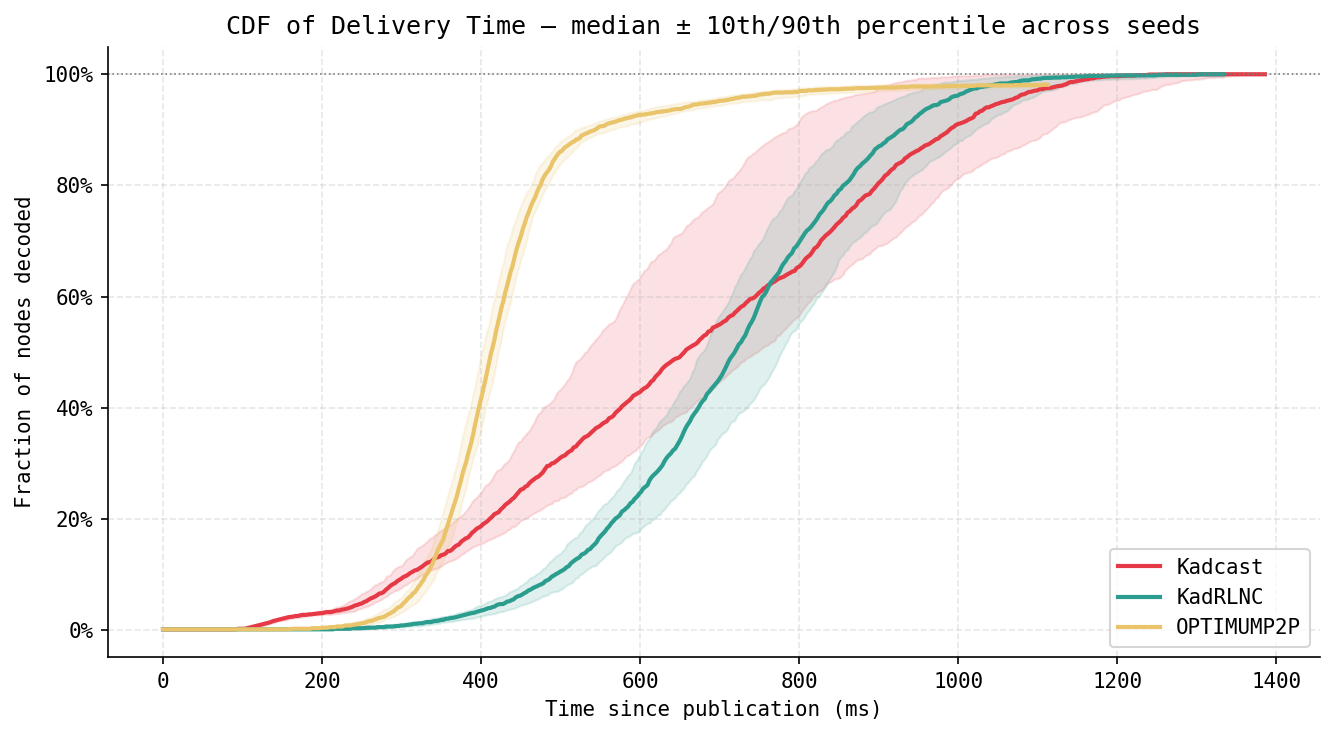
\includegraphics[width=0.8\textwidth]{base/cdf_delivery.png}
  \label{fig:base_cdf}
\end{figure}

\begin{figure}[H]
  \centering
  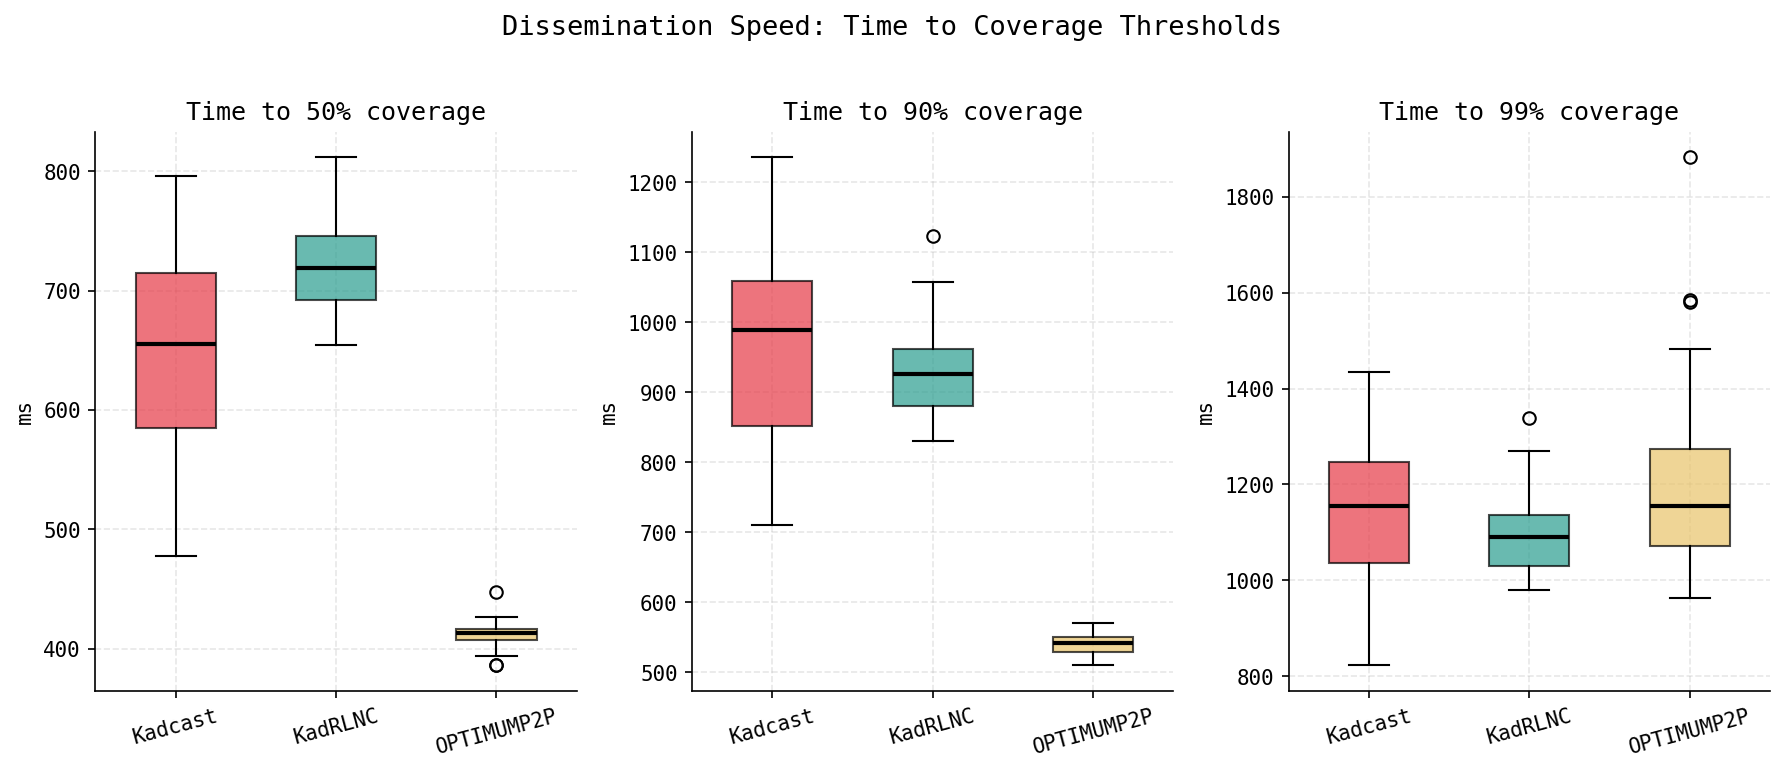
\includegraphics[width=\textwidth]{base/coverage_boxplots.png}
  \label{fig:base_box}
\end{figure}

\begin{figure}[H]
  \centering
  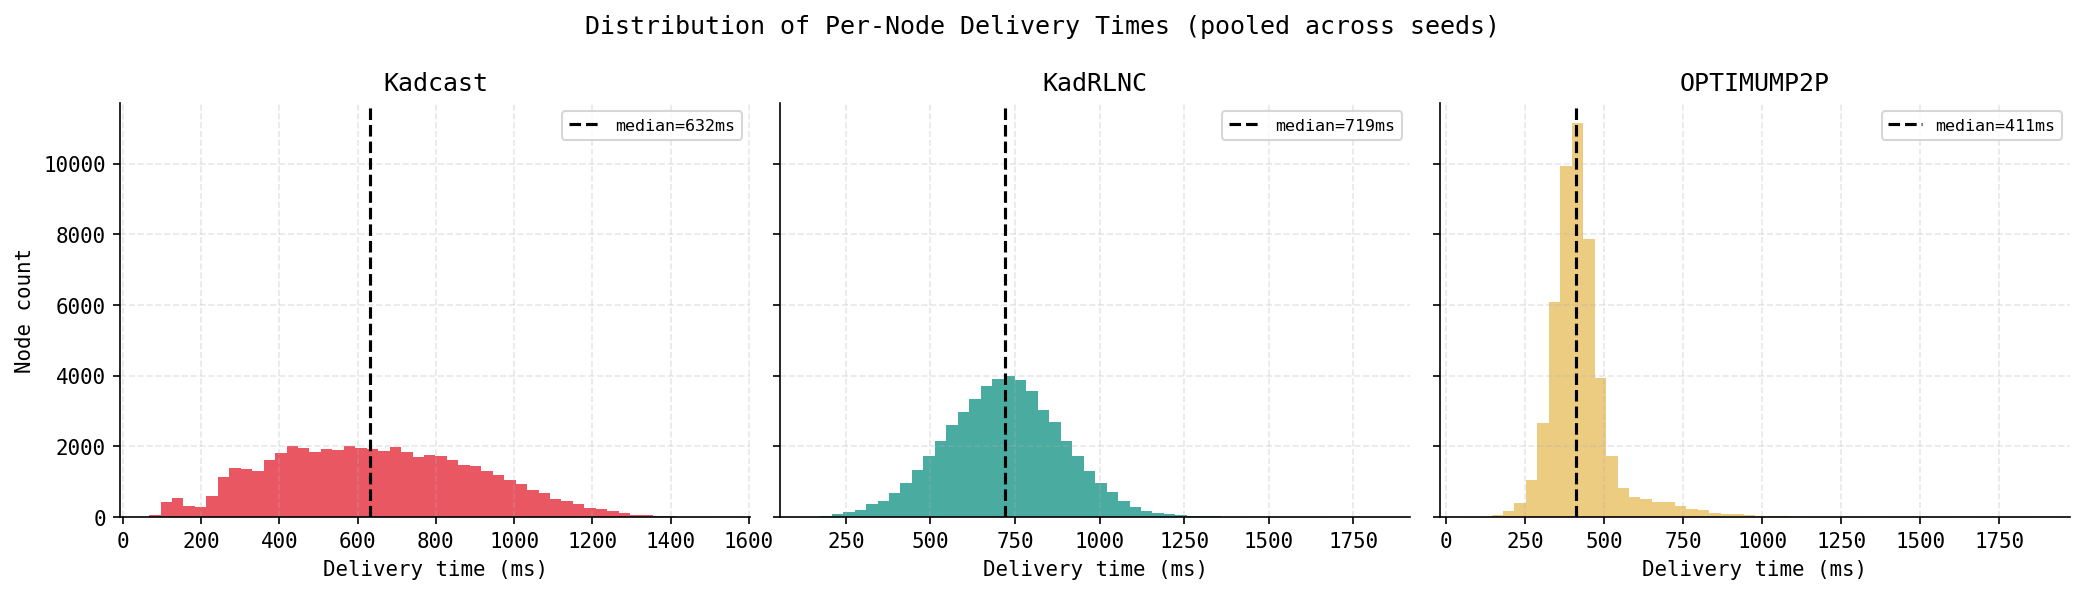
\includegraphics[width=\textwidth]{base/delivery_histograms.png}
  \label{fig:base_histo}
\end{figure}

\subsubsection*{Payload Scaling}
\begin{figure}[H]
  \centering
  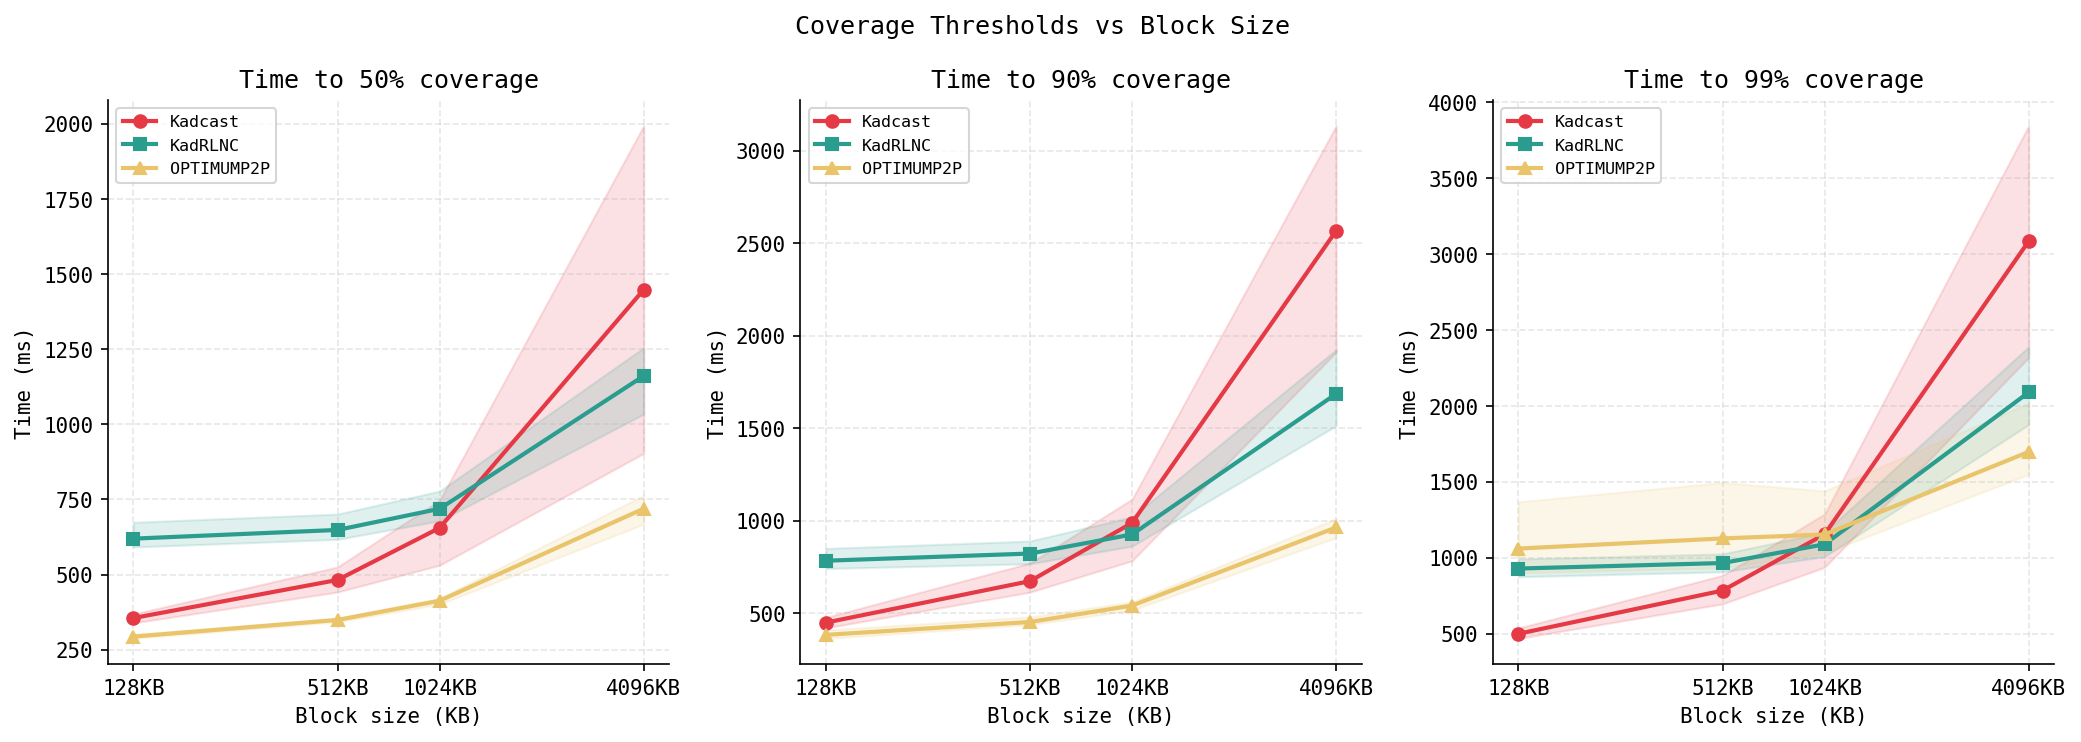
\includegraphics[width=\textwidth]{size/size_coverage_thresholds.png}
  \label{fig:size_cover}
\end{figure}

\begin{figure}[H]
  \centering
  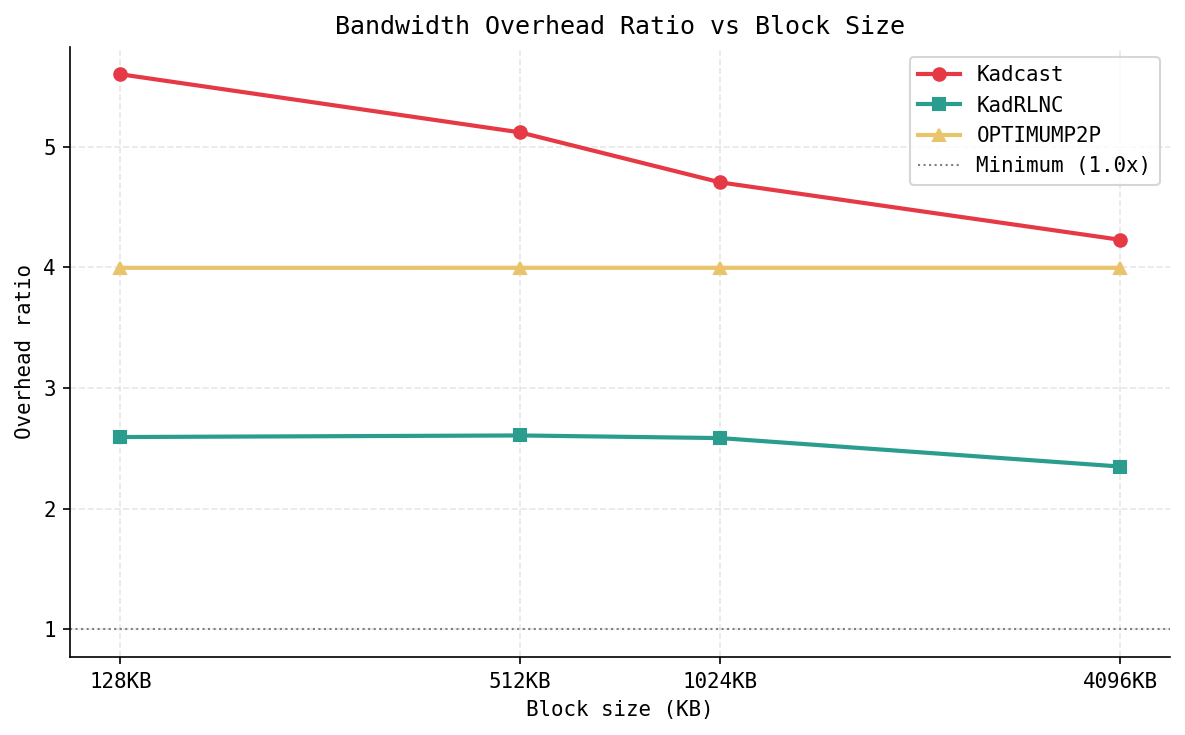
\includegraphics[width=0.7\textwidth]{size/size_overhead.png}
  \label{fig:size_overhead}
\end{figure}

\subsubsection*{Publish rate stress test}
\begin{figure}[H]
  \centering
  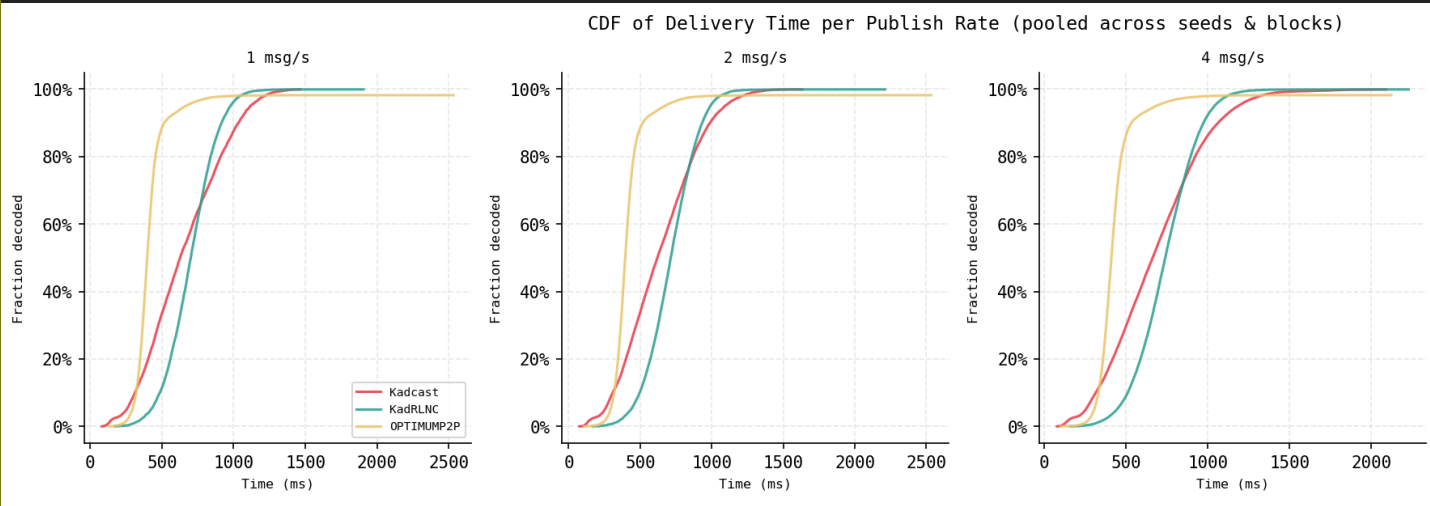
\includegraphics[width=\textwidth]{rate/rate_cdf.png}
  \label{fig:rate_cdf}
\end{figure}

\begin{figure}[H]
  \centering
  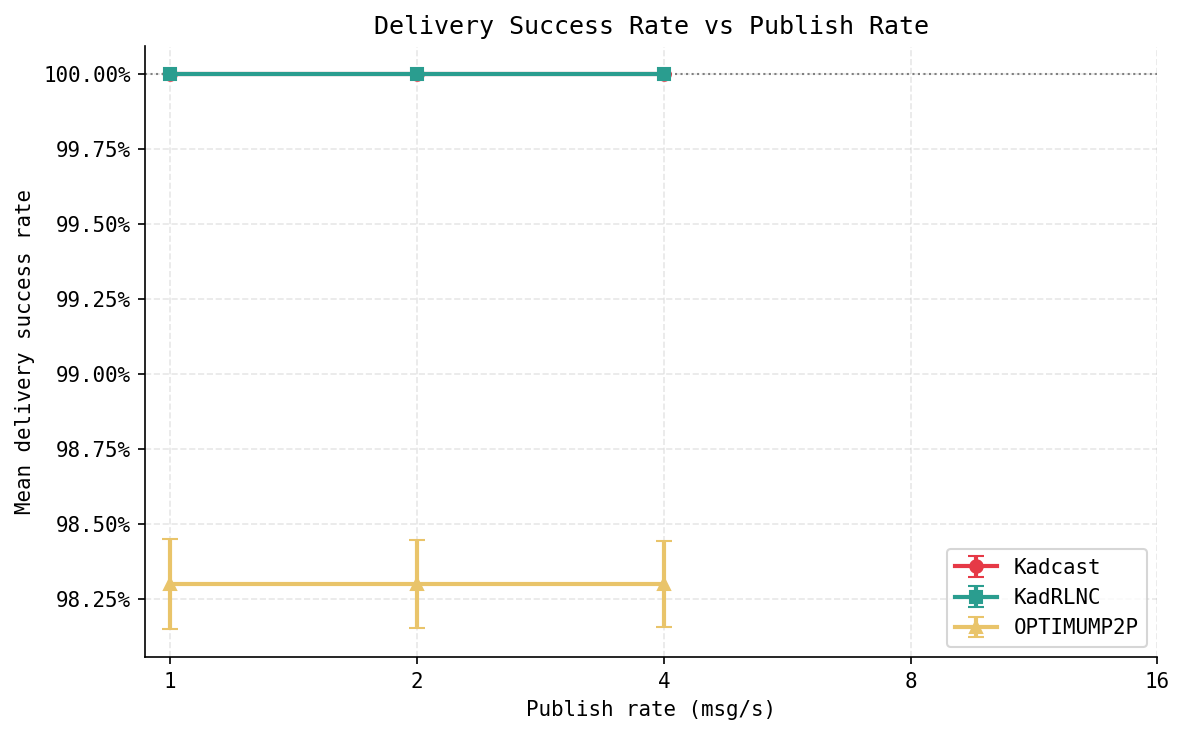
\includegraphics[width=0.7\textwidth]{rate/rate_success.png}
  \label{fig:rate_succes}
\end{figure}


\section{Conclusion}
This project set out to study information propagation in blockchain networks with the goal of understanding the design space of broadcast protocols and evaluating whether a hybrid of structured routing and network coding could improve on existing approaches.

Kadcast achieves $\Theta(\log N)$ hop depth by exploiting the Kademlia XOR-tree, but its store-and-forward relay creates a hard subtree starvation vulnerability. Optimump2p achieves excellent delivery rates through RLNC-coded push-pull gossip, but is topology-agnostic. Its stopping time $O(k + T)$ is only as good as the underlying mesh diameter $T$. KadRLNC was proposed as a hybrid that addresses both failure modes simultaneously, using $G_\text{kad}$ to structurally pin the broadcast diameter to $O(\log N)$ and RLNC to allow partial shard pooling across disrupted relay paths, with a theoretical stopping time of $O(k + \log^2 N)$.

The simulation results are more nuanced than the theory predicts. Optimump2p was the fastest protocol at the 50\% and 90\% coverage thresholds (median $\approx$410\,ms vs $\approx$720\,ms for KadRLNC in baseline dissemination), and all three protocols maintain near-100\% delivery success under publish-rate stress up to 8\,msg/s. KadRLNC's genuine empirical advantage is in bandwidth efficiency. It achieves the lowest overhead ratio ($\approx2.5\times$) across all block sizes, compared to $\approx 4\times$ for Optimump2p and up to $\approx5.5\times$ for Kadcast at small blocks and it scales more gracefully than Kadcast under increasing payload. The failure of KadRLNC to outperform Optimump2p on latency is likely a scale artefact: at $N = 1000$ with 16-bit identifiers, the Kademlia graph has only 16 buckets, and the structural diameter advantage of $G_\text{kad}$ too small to overcome the fixed 5\,ms RLNC processing overhead per node.

Several important limitations qualify these findings. The simulator uses precomputed routing tables with full global knowledge, excludes churn and adversarial behaviour, and models heterogeneity through only two static bandwidth tiers. Future work should evaluate KadRLNC at scales where $D_\text{gossip} \gg \log N$ is the realistic regime, introduce dynamic churn and Byzantine node models, and isolate the contribution of heterogeneity-aware relay selection as an independent experimental variable.

\bibliography{references}

\end{document}
